\documentclass[11pt,letterpaper]{article}

\usepackage{textcomp,marvosym}
\usepackage{amsmath,amssymb}
\usepackage[left]{lineno}
\usepackage{changepage}
\usepackage{rotating}
\usepackage{natbib}
\usepackage{setspace}
\usepackage{fancyhdr}
\usepackage{graphicx}
\usepackage[aboveskip=1pt,labelfont=bf,labelsep=period,justification=raggedright,singlelinecheck=off]{caption}
%\doublespacing

\raggedright
\textwidth = 6.5 in
\textheight = 8.25 in
\oddsidemargin = 0.0 in
\evensidemargin = 0.0 in
\topmargin = 0.0 in
\headheight = 0.0 in
\headsep = 0.5 in
\parskip = 0.1 in
\parindent = 0.2in

%\pagestyle{myheadings}
%\pagestyle{fancy}
%\fancyhf{}
%\lhead{Swanson-Hysell et al., to be submitted to GEOLOGY}
%\rhead{\thepage}

\begin{document}

\begin{flushleft}
{\Large \textbf{Data repository for ``Primary red bed magnetization revealed by fluvial intraclasts''}}

\end{flushleft}

\section*{Study location}
The study site in the Freda Formation along the Bad River is within the Ashland Syncline (Fig. \ref{fig:location_figure}A,B). There is a lack of mineralization in the Nonesuch Formation in the Ashland Syncline in contrast with localities $\sim$90 km to the east in the White Pine region \citep{Stewart2017a}. These outcrop exposures along the Bad River are very fresh as the soil-rock interface dates to retreat from the last glacial maximum which is constrained locally to be 13.2 $\pm$ 0.4 thousand years ago based on nearby $^{10}$Be exposure dates \citep{Ullman2015a}. The outcrops have been subsequently been exposed through ongoing river incision (Fig. \ref{fig:location_figure}C).

\begin{figure}[!ht]
\noindent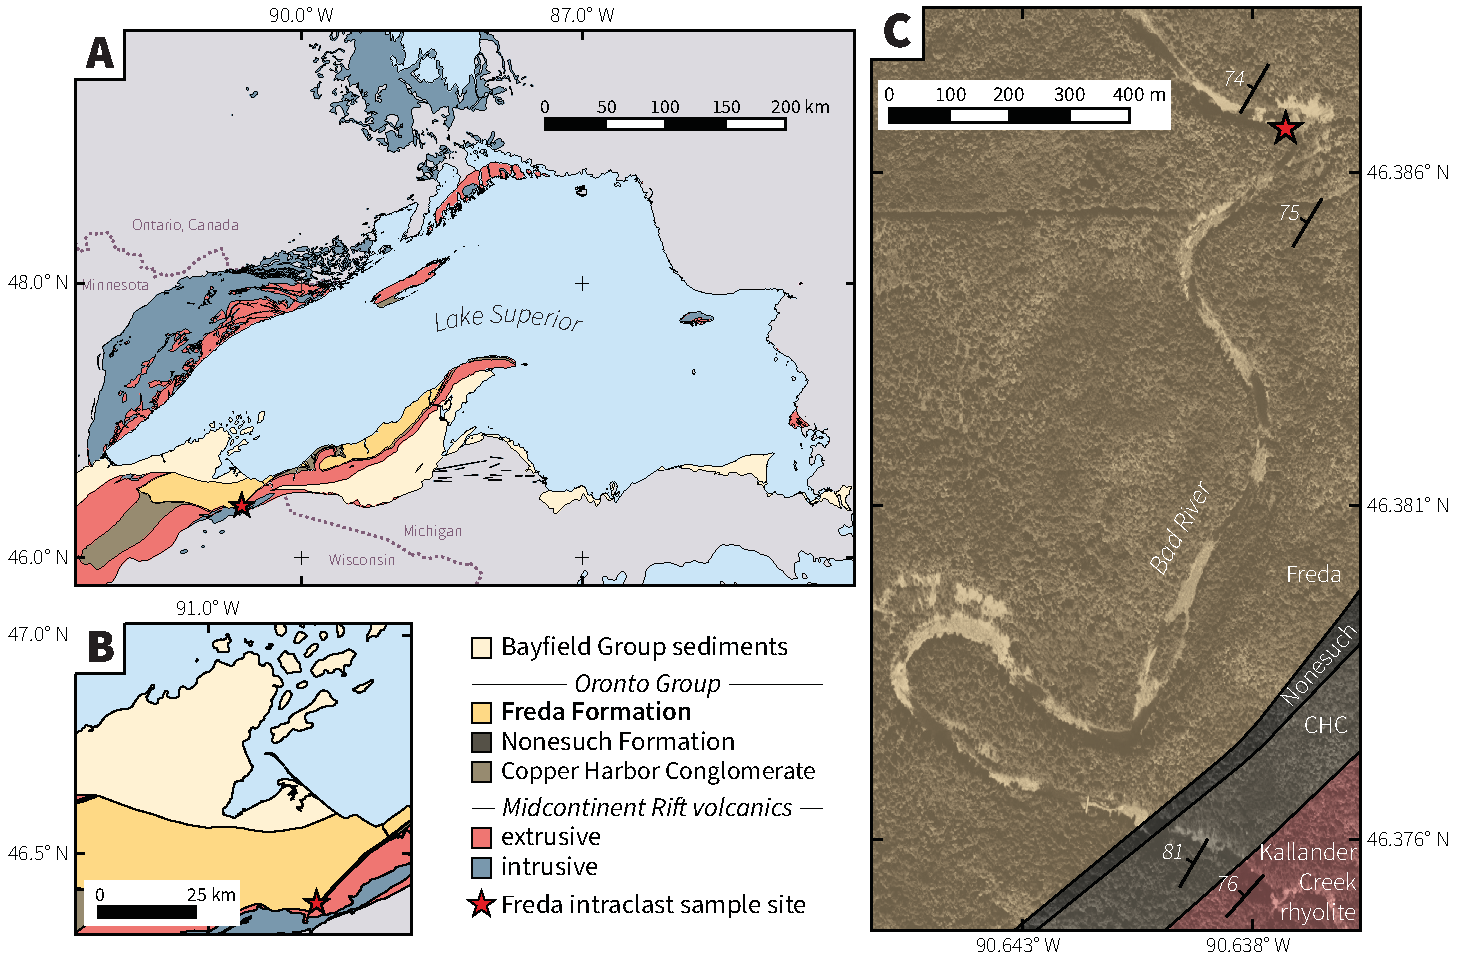
\includegraphics[width=\textwidth]{location_figure.pdf}
\caption{\small{Geological maps of the study region highlighting bedrock units associated with the Midcontinent Rift. The study location is shown as a red star on the Lake Superior region overview map (A), the zoom-in map of the eastern Ashland sycline (B) and the Bad River for which the geology is overlain on a satellite image (Esri World Imagery\nocite{Esria}). CHC stands for Copper Harbor Conglomerate. The geology has been modified from the \cite{Survey2011a}, \cite{Nicholson2004a}, and \cite{Jirsa2011a}.}}
\label{fig:location_figure}
\end{figure} 

\singlespacing

\newpage

\bibliographystyle{gsabull}
\bibliography{../../../0000_Github/references/allrefs}

\end{document}
